% !TeX program = pdflatex
% !TeX encoding = UTF-8
% Relatório v1 (rascunho parcial): resumo e seção de projeto.
\documentclass[a4paper,12pt]{article}
\usepackage[codigo,tikz]{relatorio}
\makeatletter\g@addto@macro{\UrlBreaks}{\UrlOrds}\makeatother
\setstretch{1.15}

\disciplina{Sistemas Paralelos e Distribuídos}
\professor{Ricardo Rios}
\titulo{Logística Distribuída de Soros Antivenenos}
\cabecalho{Logística distribuída de soros antivenenos}
\autor{Cristiano Peniche Ceccon}
\autor{João Victor Mattos Lopes}
\autor{Thiago Cordeiro de Melo}
\data{\today}
\descricao{%
  Relatório, primeira versão. Rascunho com o resumo e a seção de projeto do sistema.}

\begin{document}
\iniciarPreTextual
\fazcapa
\fazfolhaderosto

\begin{resumo}
O Ministério da Saúde distribui o soro antiveneno aos estados, e cada estado repassa as
ampolas a polos regionais, hospitais, postos e polos base indígenas. Essa parte da cadeia
é organizada por planilha, e-mail, telefone e rádio, e nenhum sistema mostra quantas
ampolas cada ponto tem. O resultado é soro sobrando num lugar e faltando em outro, lotes
que vencem sem ser remanejados e pacientes encaminhados para onde o soro já acabou.

Este trabalho apresenta um sistema distribuído em que cada unidade da rede estadual roda
como um nó independente, com servidor web e banco de dados próprios. As unidades registram
estoque, remessas e atendimentos localmente e trocam os dados com as vizinhas por
anti-entropia. Todo dado é um evento imutável numerado pela unidade de origem, e cada nó
resume o que tem por um vetor de versões; com isso a junção dos dados não tem conflito e
todos os nós chegam ao mesmo estado. Sobre essa base o sistema sugere reposição sem
mandar soro repetido, avisa lotes perto de vencer, detecta aumento anormal de casos por
região com o método C2 e mostra ao cidadão o caminho até o posto mais próximo com soro,
por rio, estrada ou avião. O cálculo de quais postos não podem ficar sem soro é feito em
paralelo.

Numa rede de oito nós com o exemplo do Amazonas, os postos continuaram registrando com o
polo fora do ar, todos os nós ficaram com os mesmos dados em menos de dois segundos depois
da volta, nenhum atendimento foi perdido ou duplicado e o cálculo paralelo ficou 3,9 vezes
mais rápido com 16 processos.
\palavraschave{sistemas distribuídos; replicação; vetor de versões; anti-entropia;
soro antiveneno; computação paralela}
\end{resumo}

\sumario
\iniciarTextual

\section{Projeto do sistema}
\label{sec:projeto}

\subsection{Escopo}

O sistema começa quando o soro chega ao estado. A cota mensal do Ministério da Saúde é
registrada como entrada de estoque na secretaria estadual; a compra e o envio pelo
Ministério ficam fora. Dali para baixo, a secretaria abastece polos regionais e cada polo
abastece os pontos de soro da sua região. O exemplo usado é o Amazonas: FVS-RCP em Manaus,
polos em Tabatinga e Tefé e cinco pontos de soro, incluindo um polo base indígena.
Qualquer outro estado usa o mesmo código com um arquivo de configuração próprio.

O sistema tem seis funções no escopo do semestre: estoque por lote em cada unidade,
remessas e pedidos entre os níveis, registro de atendimentos, alerta de surto por região,
painel estadual e cálculo de postos críticos. Há ainda uma tela pública em que o cidadão
vê onde há soro mais perto. Login, relatórios e exportação para os sistemas oficiais
(SIES, Sinan e SI-PNI) ficam para depois.

\subsection{Arquitetura}

Cada unidade é um nó: um processo com servidor HTTP (FastAPI com uvicorn), banco SQLite próprio, uma thread que
sincroniza com as unidades vizinhas e, nos polos e na secretaria, uma thread que verifica
surtos. A Figura~\ref{fig:topologia} mostra os nós do exemplo e os pares que sincronizam
diretamente. A hierarquia de abastecimento segue a distribuição real, mas a sincronização
pode ter atalhos: Benjamin Constant e Atalaia do Norte trocam dados entre si, e por isso
continuam se vendo se o polo cair.

\begin{figure}[htbp]
  \centering
  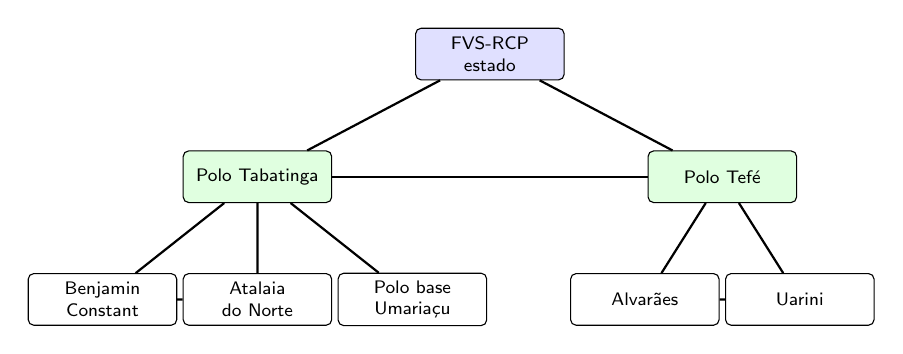
\begin{tikzpicture}[scale=0.82, every node/.style={transform shape},
      font=\sffamily\footnotesize,
      no/.style={draw, rounded corners=2pt, minimum width=2.3cm, minimum height=0.8cm, align=center, fill=#1},
      no/.default=white]
    \node[no=blue!12]  (fvs) at (0,0)      {FVS-RCP\\estado};
    \node[no=green!12] (tab) at (-3.6,-1.9) {Polo Tabatinga};
    \node[no=green!12] (tef) at (3.6,-1.9)  {Polo Tefé};
    \node[no] (bc)  at (-6.0,-3.8) {Benjamin\\Constant};
    \node[no] (ata) at (-3.6,-3.8) {Atalaia\\do Norte};
    \node[no] (uma) at (-1.2,-3.8) {Polo base\\Umariaçu};
    \node[no] (alv) at (2.4,-3.8)  {Alvarães};
    \node[no] (uar) at (4.8,-3.8)  {Uarini};
    \foreach \a/\b in {fvs/tab, fvs/tef, tab/tef, tab/bc, tab/ata, tab/uma, bc/ata, tef/alv, tef/uar, alv/uar}
      \draw[thick] (\a) -- (\b);
  \end{tikzpicture}
  \caption{Nós do exemplo do Amazonas. Cada linha liga dois nós que sincronizam
  diretamente. A secretaria abastece os polos e os polos abastecem os pontos de soro.}
  \label{fig:topologia}
\end{figure}

Usamos um nó por unidade, e não um servidor central, porque os dados nascem em muitos
lugares, mudam ao mesmo tempo e o registro no posto não pode parar se o servidor da
secretaria cair, faltar energia ou a conexão falhar. Pelo teorema CAP, durante uma
partição o sistema precisa escolher entre recusar operações ou aceitá-las e acertar
depois~\cite{gilbert2002}. Escolhemos aceitar, com a garantia de que os nós convergem.
Consenso (Raft, Paxos) e blockchain foram descartados porque exigem uma maioria de nós
conectados para gravar.

\subsection{Modelo de dados}

Todo dado é um evento imutável num diário: entrada ou saída de estoque, atendimento,
remessa, confirmação de recebimento, pedido e alerta. Cada evento tem a unidade de origem
e um número de sequência dado por ela (1, 2, 3...). O estado mostrado nas telas é
calculado a partir dos eventos: o saldo de um lote é a soma das quantidades dos movimentos
daquele lote, uma remessa está em trânsito enquanto não existe a confirmação de
recebimento, e o uso mensal é a média das saídas para atendimento nos últimos 90 dias.

Só a própria unidade grava movimentos do seu estoque: quem envia grava a saída e quem
recebe grava a entrada. Dentro do nó, as operações que leem e depois gravam o saldo passam
por uma trava. Assim, mesmo com várias pessoas usando o mesmo posto, o saldo nunca fica
negativo.

\subsection{Sincronização}

Cada nó resume os eventos que tem por um vetor de versões, que diz, para cada unidade de
origem, o maior número de sequência conhecido. Um nó só aceita o evento $n$ de uma origem
se já tem o $n-1$, e grava cada lote recebido numa única transação. Com isso ele sempre
guarda uma sequência contínua de cada origem, e o vetor descreve exatamente o que ele tem.

A cada dois segundos, com variação aleatória, o nó escolhe um vizinho e faz uma troca em
duas etapas (anti-entropia \emph{push-pull}~\cite{demers1987}): envia o seu vetor, recebe
os eventos que lhe faltam junto com o vetor do vizinho, e então envia o que falta ao
vizinho. Se o vizinho não responde, o nó tenta outro na rodada seguinte.

A convergência vem de três fatos. Os eventos não mudam depois de criados; juntar dois
diários é fazer a união de dois conjuntos, operação comutativa, associativa e idempotente,
como num CRDT do tipo conjunto que só cresce~\cite{shapiro2011}; e o estado derivado usa
somas e uniões, que não dependem da ordem de chegada. O horário dos eventos é usado só para
estatística e para mostrar há quanto tempo cada dado foi atualizado.

O atendimento leva um identificador gerado no navegador. Se a mesma requisição chegar duas
vezes, o nó devolve o atendimento já gravado e não dá baixa de novo no soro.

\subsection{Funções sobre os dados replicados}

A sugestão de reposição soma o que o destino tem com o que já está a caminho, não sugere
nada enquanto houver remessa sem confirmação e nunca passa do espaço livre da geladeira do
destino. Essa regra veio do protótipo anterior, em que o polo mandava soro repetido para
um posto isolado porque não via o recebimento.

O alerta de surto usa o método C2 do EARS~\cite{hutwagner2003}: compara os casos do dia com
a média dos sete dias que terminam três dias antes e dispara quando passa de três
desvios-padrão. Como casos de postos isolados chegam atrasados, os últimos dias são
reavaliados a cada rodada. O identificador do alerta depende só da região e da semana, de
modo que polo e secretaria geram o mesmo alerta quando detectam o mesmo surto.

A busca do cidadão usa um mapa com localidades, coordenadas e trechos com tempo e meio de
transporte (barco, voadeira, estrada, avião). O caminho é calculado pelo algoritmo de
Dijkstra no próprio sistema, sem API externa, porque os serviços comerciais de rota só
conhecem estradas. O desenho na tela usa Leaflet com o fundo do OpenStreetMap, gratuitos e
sem chave; sem internet, a página mostra um mapa esquemático e a busca continua funcionando.

\subsection{Parte paralela}

Para descobrir quais postos não podem ficar sem soro, o sistema calcula, para cada posto,
quantas comunidades hoje a até seis horas de algum soro passariam a ficar mais longe sem
ele. Cada uma dessas simulações é um Dijkstra de múltiplas origens independente das
outras. Elas são divididas em blocos e distribuídas num conjunto de processos
(\texttt{ProcessPoolExecutor}); o grafo é enviado uma vez a cada processo. Usamos
processos porque o interpretador Python executa uma thread de cada vez em código puro.

\subsection{Avaliação preliminar}

O comando \texttt{python -m soro avaliar} sobe os oito nós em processos separados e mede
as quatro perguntas definidas na proposta. A Tabela~\ref{tab:avaliacao} resume uma
execução num notebook com processador Intel i7-12700H.

\begin{table}[htbp]
  \centering
  \caption{Resultados de uma execução da avaliação (sincronização a cada 0,5 s).}
  \label{tab:avaliacao}
  \small
  \begin{tabularx}{\textwidth}{>{\raggedright\arraybackslash}p{3.2cm}X>{\raggedright\arraybackslash}p{4.2cm}}
    \toprule
    Pergunta & Como foi medida & Resultado \\
    \midrule
    Falha de um nó & Polo Tabatinga encerrado; 10 atendimentos em cada posto dele & 30 de 30 aceitos; nós iguais 1,7 s depois da volta do polo \\
    Dados iguais & 20 atendimentos ao mesmo tempo em cada um dos 8 nós & mesmo resumo em todos em 1,7 s \\
    Nada se perde & 10 atendimentos reenviados duas vezes; contagem em todos os nós & 200 casos distintos em cada nó \\
    Velocidade & Postos críticos num mapa de 14.400 localidades e 200 postos & 7,9 s com 1 processo e 2,0 s com 16 (3,9 vezes) \\
    \bottomrule
  \end{tabularx}
\end{table}

O ganho do paralelismo para perto de quatro vezes porque o processador do notebook reduz a
frequência sob carga e mistura núcleos de desempenho e de eficiência. A próxima etapa vai
comparar o sistema com uma versão centralizada e contar quantos registros ela recusaria em
cada queda.

\footnotesize
\begin{thebibliography}{9}
\addcontentsline{toc}{section}{Referências}
\bibitem{gilbert2002} GILBERT, S.; LYNCH, N. Brewer's conjecture and the feasibility of
  consistent, available, partition-tolerant web services. \textit{SIGACT News}, 2002.
\bibitem{demers1987} DEMERS, A. et al. Epidemic algorithms for replicated database
  maintenance. In: \textit{ACM PODC}, 1987.
\bibitem{shapiro2011} SHAPIRO, M. et al. Conflict-free replicated data types.
  \textit{SSS}, LNCS 6976, 2011.
\bibitem{hutwagner2003} HUTWAGNER, L. et al. The bioterrorism preparedness and response
  Early Aberration Reporting System (EARS). \textit{J. Urban Health}, 2003.
\end{thebibliography}

\end{document}
